\documentclass[a4paper,fleqn]{cas-sc}
\usepackage[numbers,sort&compress]{natbib}
\usepackage{fontspec}
\setmainfont{DejaVuSerif.ttf}[Path=fonts/,BoldFont=DejaVuSerif-Bold.ttf,ItalicFont=DejaVuSerif.ttf,ItalicFeatures={FakeSlant=0.18},BoldItalicFont=DejaVuSerif-Bold.ttf,BoldItalicFeatures={FakeSlant=0.18}]
\setsansfont{DejaVuSans.ttf}[Path=fonts/,BoldFont=DejaVuSans-Bold.ttf,ItalicFont=DejaVuSans.ttf,ItalicFeatures={FakeSlant=0.18}]
\setmonofont{Latin Modern Mono}[Scale=MatchLowercase]
\usepackage{tabularx,longtable,enumitem,placeins,fvextra,fix-cm}
\usepackage[font=small,labelfont=bf]{caption}
\geometry{a4paper,top=20mm,bottom=25mm,left=20mm,right=20mm,headsep=10pt,footskip=26pt}
% Thong tin co the sua. Bien dich bang XeLaTeX.
\newcommand{\StudentName}{Đặng Trung Hiếu}
\newcommand{\UniversityName}{Trường Đại học Công nghệ, Đại học Quốc gia Hà Nội}
\newcommand{\ReportDate}{17/10/2026}
% Dien URL that khi da dua ma nguon va du lieu len kho luu tru.
% Vi du cu phap: \newcommand{\CodeURL}{https://...}
\newcommand{\CodeURL}{}
\newcommand{\DataURL}{}
\newcommand{\ShowCodeURL}{\ifdefempty{\CodeURL}{\textbf{Chưa bổ sung URL mã nguồn.}}{\expandafter\url\expandafter{\CodeURL}}}
\newcommand{\ShowDataURL}{\ifdefempty{\DataURL}{\textbf{Chưa bổ sung URL dữ liệu thô.}}{\expandafter\url\expandafter{\DataURL}}}

\renewcommand{\figurename}{Hình}
\renewcommand{\tablename}{Bảng}
\renewcommand{\refname}{Tài liệu tham khảo}
\renewcommand{\abstractname}{TÓM TẮT}
\setlength{\emergencystretch}{2em}
\setlength{\parskip}{2pt}
\setlist[itemize]{leftmargin=1.5em,itemsep=1pt,topsep=3pt}
\setlist[enumerate]{leftmargin=1.7em,itemsep=1pt,topsep=3pt}
\newcommand{\AMO}{\operatorname{AMO}}
\newcommand{\ALO}{\operatorname{ALO}}
\newcommand{\EO}{\operatorname{EO}}
\newcommand{\AllDifferent}{\operatorname{AllDifferent}}
\newcommand{\code}[1]{\texttt{\detokenize{#1}}}
\newcommand{\TO}{\textsf{TO}}
\newcommand{\GL}{\textsf{GL}}
\newcommand{\tabnote}[1]{\par\vspace{3pt}{\footnotesize #1\par}}
\newtheorem{proposition}{Mệnh đề}
\newcounter{algorithm}
\ExplSyntaxOn
% CAS uses a zero-width box for the left keyword column; absorb its deliberate
% extension with hss so the box has its correct intended width without warnings.
\RenewDocumentEnvironment{Abstract}{o}
 {
  \group_begin:
  \IfNoValueTF{#1}{}{\tex_gdef:D\abstractname{#1}}
  \parindent=0pt
  \box_if_empty:NTF\g_stm_key_box
   {\leftskip=.35\textwidth}
   {
    \dim_gset:Nn\l_tmpa_dim{\box_ht:N\g_stm_key_box}
    \dim_gadd:Nn\l_tmpa_dim{\box_dp:N\g_stm_key_box}
    \leftskip=.35\textwidth
    \hspace*{-.35\textwidth}
    \noindent\hbox_to_wd:nn{0pt}{\box\g_stm_key_box\hss}
    \skip_vertical:n{-\l_tmpa_dim}
   }
  \noindent\abstractname\par
  \skip_vertical:n{-4pt}
  \noindent\rule{.65\textwidth}{.2pt}\par\footnotesize
  \ignorespaces\everypar{\parindent=1.5em}
 }
 {\par\group_end:}
\RenewDocumentCommand\printorcid{}{}
\cs_gset:Npn \__first_footerline:
 {\small\sffamily Bài~tập~lớn~1~|~Bản~thảo~\ReportDate}
\cs_gset:Npn \__first_foot:
 {\parbox[t]{\textwidth}{\rule{\textwidth}{.2pt}\\\__first_footerline:\hfill Trang~\thepage/\lastpage}}
\cs_gset:Npn \__cas_foot:
 {\parbox[t]{\textwidth}{\rule{\textwidth}{.2pt}\\\__first_footerline:\hfill Trang~\thepage/\lastpage}}
\ExplSyntaxOff
\hypersetup{pdftitle={Giải bài toán N-Queens bằng SAT: mã hóa và đánh giá thực nghiệm},pdfauthor={Đặng Trung Hiếu},pdfsubject={Bài tập lớn 1 - Các vấn đề hiện đại KHMT},pdfproducer={XeLaTeX}}

\begin{document}
\pagestyle{cas}
\let\WriteBookmarks\relax
\shorttitle{N-Queens bằng SAT: mã hóa và đánh giá thực nghiệm}
\shortauthors{Đặng Trung Hiếu}
\title[mode=title]{Giải bài toán N-Queens bằng SAT:\texorpdfstring{\\}{ }mã hóa và đánh giá thực nghiệm}
\author[1]{\StudentName}
\affiliation[1]{organization={\UniversityName},city={Hà Nội},country={Việt Nam}}
\nonumnote{Bài tập lớn 1, học phần Các vấn đề hiện đại KHMT, học kỳ I năm học 2026--2027. Bản thảo ngày \ReportDate; cần bổ sung hai liên kết ở mục Data Availability trước khi nộp.}
\begin{abstract}
Báo cáo xây dựng bộ giải N-Queens bằng thư viện PySAT với Glucose3 và ba mã hóa ràng buộc tối đa một: pairwise, sequential counter và bitwise. Mô hình dùng một biến Boolean cho mỗi ô, ràng buộc đúng một quân hậu trên mỗi hàng, mỗi cột và tối đa một trên mỗi đường chéo. Tính đúng đắn được chứng minh theo hai chiều giữa nghiệm bàn cờ và mô hình SAT. Thực nghiệm so sánh ba cấu hình SAT với OR-Tools CP-SAT, IBM CP Optimizer, CPLEX MIP và Gurobi MIP trên bảy kích thước từ 8 đến 128, mỗi cấu hình lặp năm lần, giới hạn pha giải 30 giây. Trong 220 lượt thực sự gọi solver, 210 lượt trả về nghiệm hợp lệ và 10 lượt hết thời gian; 25 lượt khác được bỏ qua theo chính sách giấy phép. Không có mã hóa SAT tốt nhất trên mọi kích thước. Tại $N=128$, bitwise có trung vị tổng thời gian 1,074 giây, pairwise 4,106 giây, còn sequential counter hết thời gian ở cả năm lượt. Mặc dù pairwise tạo hơn 3,46 triệu mệnh đề, phần lớn thời gian của cấu hình này nằm ở dựng và nạp CNF. IBM CP Optimizer có trung vị thấp nhất trong các cấu hình đã chạy ở $N=32,64,128$. Kết quả cho thấy cần đánh giá cả kích thước biểu diễn, chi phí chuẩn bị và quá trình tìm kiếm; kết luận chỉ áp dụng cho cấu hình và tập bàn cờ đã khảo sát.
\end{abstract}
\begin{keywords}[Từ khóa]
N-Queens \sep SAT \sep PySAT \sep cardinality encoding \sep CP-SAT \sep thực nghiệm
\end{keywords}
\maketitle
\hypersetup{pdftitle={Giải bài toán N-Queens bằng SAT: mã hóa và đánh giá thực nghiệm},pdfauthor={Đặng Trung Hiếu},pdfsubject={Bài tập lớn 1 - Các vấn đề hiện đại KHMT}}

\section{Giới thiệu}\label{sec:intro}
Bài toán N-Queens yêu cầu đặt $N$ quân hậu trên bàn cờ $N\times N$ sao cho không có hai quân hậu tấn công nhau. Quy tắc ngắn gọn nhưng có thể được biểu diễn bằng nhiều mô hình: mệnh đề Boolean, biến nguyên với ràng buộc toàn cục, hoặc quy hoạch nguyên nhị phân. Vì vậy, đây là một bài toán phù hợp để thực hành chuyển yêu cầu logic thành ràng buộc và khảo sát ảnh hưởng của cách biểu diễn tới một bộ giải cụ thể.

Phạm vi của báo cáo là \emph{tìm một nghiệm của N-Queens chuẩn}: bàn cờ không có ô cấm và không đặt sẵn quân hậu. Bài toán có nghiệm với $N=1$ và mọi $N\geq4$, không có nghiệm với $N=2,3$. Không nên gọi bài toán quyết định này là NP-complete. Kết quả NP-complete của Gent và cộng sự áp dụng cho \emph{N-Queens Completion}, nơi một phần quân hậu đã được cố định \citep{gent2017}. Báo cáo không xét bài toán đếm hay liệt kê toàn bộ nghiệm.

Với SAT, hai công thức biểu diễn cùng một bài toán vẫn có thể khác rất nhiều về số biến phụ, số mệnh đề và thời gian tìm kiếm. PySAT cung cấp giao diện chung tới các SAT solver cùng các bộ mã hóa cardinality, giúp khảo sát yếu tố này trong một chương trình Python thống nhất \citep{pysat2018}. Ở đây, Glucose3 được giữ cố định và chỉ thay mã hóa AMO. Các phương pháp CP và MIP được dùng làm đối chứng theo yêu cầu của bài tập lớn, với các giới hạn phần mềm được công bố rõ.

Báo cáo tập trung vào ba câu hỏi:
\begin{enumerate}
\item Ba mã hóa AMO làm thay đổi số biến, số mệnh đề và thời gian giải N-Queens như thế nào?
\item Chi phí dựng và khởi tạo mô hình đóng góp bao nhiêu vào tổng thời gian, đặc biệt khi bàn cờ lớn?
\item Các cấu hình SAT thể hiện ra sao so với CP-SAT, CP Optimizer và hai bộ giải MIP trong điều kiện thực nghiệm hiện có?
\end{enumerate}
Đóng góp của bài tập là một quy trình mô hình hóa, giải mã và kiểm tra nghiệm; một cơ chế đo có kiểm soát thời gian ở cấp tiến trình; và bộ kết quả có thể đối chiếu với dữ liệu thô. Đây là đánh giá các cài đặt cụ thể, không phải đề xuất thuật toán SAT mới hay xếp hạng tổng quát các họ solver.

\section{Cơ sở và các mô hình đối chứng}\label{sec:background}
\subsection{Định nghĩa và ký hiệu}
Đánh số hàng và cột từ $0$ đến $N-1$. Một nghiệm là tập
\begin{equation}
 Q=\{(r,q_r):0\leq r<N\},\qquad q_r\in\{0,\ldots,N-1\},
\end{equation}
trong đó $q_r$ là cột đặt hậu ở hàng $r$. Với mọi $r\ne s$, cần có
\begin{equation}\label{eq:valid}
 q_r\ne q_s,\qquad r+q_r\ne s+q_s,\qquad r-q_r\ne s-q_s.
\end{equation}
Hai điều kiện cuối phân biệt hai họ đường chéo. Chẳng hạn, $Q=\{(0,1),(1,3),(2,0),(3,2)\}$ là nghiệm của $N=4$: các cột là $1,3,0,2$; các tổng là $1,4,2,5$; các hiệu là $-1,-2,2,1$, đều không lặp.

\subsection{SAT và ràng buộc cardinality}
Một literal là biến Boolean hoặc phủ định của nó. Mệnh đề là phép tuyển các literal; CNF là phép hội các mệnh đề. Solver tìm phép gán làm đúng toàn bộ CNF, hoặc chứng minh không tồn tại phép gán đó. Với tập biến $X=\{x_1,\ldots,x_k\}$, ký hiệu
\begin{align}
 \ALO(X)&=x_1\lor\cdots\lor x_k,\\
 \AMO(X)&\equiv\sum_{i=1}^{k}x_i\leq1,\\
 \EO(X)&=\ALO(X)\land\AMO(X).
\end{align}
ALO chỉ cần một mệnh đề. AMO có nhiều cách chuyển sang CNF; việc thêm biến phụ cho phép giảm số mệnh đề. Khi có biến phụ, tính tương đương cần hiểu theo phép chiếu: một phép gán cho các biến gốc hợp lệ khi và chỉ khi có thể mở rộng nó thành phép gán thỏa CNF.

Glucose thuộc họ solver CDCL, sử dụng học mệnh đề khi gặp xung đột. Công trình của Audemard và Simon nghiên cứu chất lượng mệnh đề học, là nền tảng của Glucose \citep{glucose2009}. Báo cáo gọi Glucose3 qua tên \code{g3} trong PySAT; không tự cài đặt lại thuật toán tìm kiếm bên trong solver.

\subsection{Mô hình biến nguyên cho CP-SAT và CP Optimizer}\label{sec:cp}
Mỗi hàng có một biến nguyên $q_r\in[0,N-1]$. Ba ràng buộc toàn cục là
\begin{equation}\label{eq:cp}
 \AllDifferent(q_r),\quad
 \AllDifferent(q_r+r),\quad
 \AllDifferent(q_r-r),\qquad 0\leq r<N.
\end{equation}
Mỗi biến biểu diễn đúng một quân hậu ở hàng tương ứng; ba ràng buộc ngăn trùng cột và đường chéo. Đây là cấu trúc mô hình được minh họa trong tài liệu chính thức của OR-Tools và DOcplex.CP \citep{ortoolsqueens,docplexcp}. Trong cài đặt, CP-SAT dùng \code{CpModel}; CP Optimizer (nhãn CPLEX CP trong biểu đồ) dùng \code{CpoModel} và runtime cục bộ.

CP-SAT là bộ giải ràng buộc số nguyên dựa trên công nghệ SAT, không nên hiểu nhãn ``CP-SAT'' là một solver CP thuần túy tách biệt hoàn toàn với SAT \citep{ortoolscpsat}. Số $N$ biến và ba ràng buộc ở đây chỉ mô tả \emph{mô hình đầu vào}; solver có thể chuyển đổi nội bộ thành biểu diễn khác. Vì thế không so sánh trực tiếp ``ba AllDifferent'' với số mệnh đề CNF như cùng một đơn vị độ phức tạp.

\subsection{Mô hình nhị phân cho CPLEX MIP và Gurobi MIP}\label{sec:mip}
Đặt $x_{r,c}\in\{0,1\}$ cho mỗi ô. Hai bộ giải dùng cùng các ràng buộc tuyến tính:
\begin{align}
 \sum_{c=0}^{N-1}x_{r,c}&=1 &&(0\leq r<N),\label{eq:miprow}\\
 \sum_{r=0}^{N-1}x_{r,c}&=1 &&(0\leq c<N),\\
 \sum_{(r,c)\in D}x_{r,c}&\leq1 &&(D\text{ là đường chéo, }|D|\geq2).
\end{align}
Hàm mục tiêu là hằng số $0$; yêu cầu thực chất là tìm một phương án khả thi. Do đó báo cáo không đánh giá giá trị mục tiêu hay khoảng cách tối ưu. Mô hình có $N^2$ biến nhị phân và $6N-6$ ràng buộc tuyến tính với $N\geq2$: $2N$ ràng buộc hàng/cột và $4N-6$ ràng buộc đường chéo. Không bổ sung phá vỡ đối xứng trong bất kỳ mô hình nào.

\section{Mã hóa N-Queens sang SAT}\label{sec:sat}
\subsection{Biến và các nhóm ràng buộc}
Biến $x_{r,c}$ đúng khi và chỉ khi có quân hậu tại ô $(r,c)$. Định danh nguyên dùng trong PySAT là
\begin{equation}\label{eq:id}
 \operatorname{id}(r,c)=rN+c+1.
\end{equation}
Như vậy các biến bàn cờ chiếm các định danh $1,\ldots,N^2$. Biến phụ được cấp từ $N^2+1$ bằng một \code{IDPool} dùng chung cho toàn bộ công thức. Dùng các bộ cấp phát riêng không phối hợp có thể làm trùng biến phụ giữa những ràng buộc độc lập và thay đổi sai ý nghĩa mô hình.

Đặt $R_r=\{x_{r,c}:0\leq c<N\}$, $C_c=\{x_{r,c}:0\leq r<N\}$ và
\begin{align}
 D^-_d&=\{x_{r,c}:r-c=d\},& -(N-1)\leq d\leq N-1,\\
 D^+_s&=\{x_{r,c}:r+c=s\},& 0\leq s\leq2N-2.
\end{align}
Với mã hóa AMO được chọn là $e$, công thức tổng thể là
\begin{equation}\label{eq:cnf}
 F_{N,e}=\bigwedge_r\EO_e(R_r)\land\bigwedge_c\EO_e(C_c)
 \land\bigwedge_{d:\,|D^-_d|>1}\AMO_e(D^-_d)
 \land\bigwedge_{s:\,|D^+_s|>1}\AMO_e(D^+_s).
\end{equation}
Đường chéo một ô không cần thêm ràng buộc. Trên hàng và cột, EO được xây dựng từ một mệnh đề ALO và CNF của AMO. Dù EO trên hàng cùng AMO trên cột đã đủ với $N$ quân hậu, cài đặt đang khảo sát vẫn dùng EO cho \emph{cả hàng lẫn cột}. Chi tiết này được giữ nguyên khi đếm mệnh đề và so sánh thực nghiệm.

\subsection{Mã hóa pairwise}
Với $k$ biến, pairwise cấm từng cặp cùng đúng:
\begin{equation}\label{eq:pair}
 \AMO_{\mathrm{pw}}(X)=\bigwedge_{1\leq i<j\leq k}(\neg x_i\lor\neg x_j).
\end{equation}
Mã hóa có $\binom{k}{2}$ mệnh đề nhị phân, không có biến phụ. Nếu hai biến cùng đúng, mệnh đề của cặp đó sai; nếu nhiều nhất một biến đúng, mọi cặp đều thỏa. Khi một biến được gán đúng, các mệnh đề chứa nó trực tiếp buộc những biến còn lại sai.

Với toàn bộ bàn cờ, hai nhóm hàng/cột tạo $2N\binom{N}{2}$ mệnh đề AMO và $2N$ mệnh đề ALO. Trong mỗi họ đường chéo, độ dài là $1,2,\ldots,N-1,N,N-1,\ldots,1$. Suy ra số mệnh đề được dựng, trước mọi biến đổi trong solver, là
\begin{align}\label{eq:paircount}
 C_{\mathrm{pw}}(N)
 &=2N+2N\binom{N}{2}+2\binom{N}{2}+4\sum_{k=1}^{N-1}\binom{k}{2}\nonumber\\
 &=\frac{5N^3-6N^2+7N}{3}.
\end{align}
Đây là công thức đếm của mô hình cụ thể ở \eqref{eq:cnf}, không phải của mọi mô hình SAT cho N-Queens. Nó cho $C_{\mathrm{pw}}(128)=3\,462\,784$, trùng dữ liệu ghi nhận.

\subsection{Mã hóa sequential counter}
Một dạng AMO của bộ đếm tuần tự Sinz dùng $k-1$ biến phụ $s_1,\ldots,s_{k-1}$ \citep{sinz2005}. Các mệnh đề, với $k\geq2$, là
\begin{align}
 &(\neg x_1\lor s_1),\qquad(\neg x_k\lor\neg s_{k-1}),\label{eq:seq}\\
 &(\neg x_i\lor s_i)\land(\neg s_{i-1}\lor s_i)\land(\neg x_i\lor\neg s_{i-1}),
 \quad 2\leq i\leq k-1.\nonumber
\end{align}
Thông tin ``đã có biến đúng ở tiền tố'' được truyền theo chuỗi; một biến đúng phía sau không thể cùng tồn tại với tiền tố đã đúng. Dạng trên dùng $3k-4$ mệnh đề, tuyến tính theo $k$, nhưng cần biến phụ. Số đếm này mô tả công thức chuẩn; thư viện có thể đơn giản hóa trường hợp nhỏ. Báo cáo dùng số mệnh đề và số biến \emph{thực sự sinh ra} để lập bảng thực nghiệm, không thay chúng bằng công thức lý thuyết.

\subsection{Mã hóa bitwise}
Gán cho mỗi $x_i$ một mã nhị phân khác nhau gồm $b=\lceil\log_2k\rceil$ bit. Thêm các biến chọn $z_1,\ldots,z_b$ và áp đặt
\begin{equation}\label{eq:bitwise}
 x_i\Rightarrow\bigwedge_{j=1}^{b}\ell_{i,j},\qquad
 \ell_{i,j}=\begin{cases}z_j&\text{nếu bit }j\text{ của mã }i\text{ là }1,\\
 \neg z_j&\text{nếu bit đó là }0.\end{cases}
\end{equation}
Mỗi kéo theo tạo các mệnh đề $(\neg x_i\lor\ell_{i,j})$. Nếu hai $x_i$ cùng đúng, hai mã khác nhau ở ít nhất một bit và gây mâu thuẫn. Nếu tất cả $x_i$ sai, các bit chọn được tự do; đây là hành vi hợp lệ của AMO. Khi cần EO, mệnh đề ALO bổ sung việc phải chọn một biến.

Dạng nhị phân trực tiếp có $b$ biến phụ và $kb$ mệnh đề. PySAT cung cấp \code{EncType.bitwise}; các đơn giản hóa có thể làm số đếm cụ thể thấp hơn mô tả trực tiếp này \citep{pysatcard}. Bitwise ở đây là mã hóa AMO bằng bit chọn, không phải thuật toán quay lui sử dụng bitmask trên bàn cờ.

\subsection{Quy mô biểu diễn và tính đúng đắn}
Bảng~\ref{tab:asymptotic} tổng hợp bậc tăng của các công thức. Có $O(N)$ nhóm ràng buộc, mỗi nhóm dài tối đa $N$; tổng độ dài các nhóm là $O(N^2)$. Do vậy pairwise có số mệnh đề bậc ba theo $N$, sequential counter có bậc hai, còn bitwise có cận $O(N^2\log N)$. Những cận này nói về \emph{kích thước đầu vào}, không phải cam kết thời gian giải.

\begin{table}[htbp]
\caption{Quy mô mã hóa toàn bàn cờ; số biến gốc luôn bằng $N^2$.}\label{tab:asymptotic}
\centering
\begin{tabular}{lccc}
\toprule
Mã hóa & Biến phụ & Tổng biến & Số mệnh đề\\
\midrule
Pairwise & $0$ & $N^2$ & $\Theta(N^3)$\\
Sequential counter & $O(N^2)$ & $O(N^2)$ & $O(N^2)$\\
Bitwise & $O(N\log N)$ & $N^2+O(N\log N)$ & $O(N^2\log N)$\\
\bottomrule
\end{tabular}
\end{table}

\begin{proposition}\label{prop:soundcomplete}
Với một bộ mã hóa AMO đúng và các biến phụ không trùng giữa các nhóm, $F_{N,e}$ thỏa được khi và chỉ khi bàn cờ $N\times N$ có một nghiệm N-Queens.
\end{proposition}
\noindent\textit{Chứng minh.}
Nếu $F_{N,e}$ có mô hình, EO trên mỗi hàng chọn đúng một ô, tạo đúng $N$ quân hậu. EO trên cột và AMO trên hai họ đường chéo cấm mọi cặp tấn công. Phép chiếu lên các biến $x_{r,c}$ vì thế cho một nghiệm hợp lệ.

Ngược lại, từ một nghiệm bàn cờ, gán đúng chính các biến của ô có hậu. Mỗi hàng và cột có đúng một hậu; mỗi đường chéo có nhiều nhất một hậu, nên tất cả ràng buộc gốc thỏa. Tính đúng của bộ mã hóa AMO bảo đảm tồn tại phép gán mở rộng cho các biến phụ của từng nhóm. Do các nhóm dùng định danh phụ riêng, có thể ghép các phép gán này thành một mô hình của toàn công thức.\hfill$\square$

\section{Thiết kế và cài đặt bộ giải}\label{sec:implementation}
\subsection{Luồng xử lý và giải mã}
Bộ giải nhận số nguyên dương $N$ và tên mã hóa. Phần dựng CNF dùng \code{CardEnc.atmost} với \code{bound=1}; các tùy chọn tương ứng là \code{pairwise}, \code{seqcounter} và \code{bitwise}. Giao diện \code{CardEnc} hỗ trợ dùng chung \code{vpool} để quản lý định danh phụ \citep{pysatcard}. CNF được nạp bằng \code{Solver(name="g3", bootstrap_with=clauses)}.

Thuật toán~\ref{alg:solver} trình bày luồng xử lý ở mức khái niệm. Với literal dương $v$ thuộc khoảng $1\leq v\leq N^2$, tọa độ được khôi phục bởi
\begin{equation}\label{eq:decode}
 r=\left\lfloor\frac{v-1}{N}\right\rfloor,\qquad c=(v-1)\bmod N.
\end{equation}
Mọi literal âm và mọi định danh biến phụ đều bị loại khỏi phép giải mã. Không được diễn giải một biến phụ đúng thành một quân hậu.

\begin{figure}[htbp]
\refstepcounter{algorithm}\label{alg:solver}
\centering
\begin{minipage}{0.96\linewidth}
\hrule\vspace{5pt}
\textbf{Thuật toán 1.} Tìm một nghiệm N-Queens bằng SAT
\begin{enumerate}
\item Kiểm tra $N$ là số nguyên dương và mã hóa $e$ được hỗ trợ.
\item Khởi tạo $N^2$ biến bàn cờ, một bộ cấp phát biến phụ và CNF rỗng.
\item Thêm EO cho từng hàng, từng cột; thêm AMO cho từng đường chéo dài hơn một ô.
\item Khởi tạo Glucose3 và nạp CNF; gọi phương thức giải.
\item Nếu solver chứng minh không thỏa: trả UNSAT. Nếu chưa có kết luận trong hạn: trả UNKNOWN.
\item Nếu SAT: chiếu mô hình lên biến bàn cờ, giải mã bằng \eqref{eq:decode}, kiểm tra nghiệm; chỉ trả SAT khi kiểm tra thành công.
\item Giải phóng tài nguyên solver và kết thúc lượt chạy.
\end{enumerate}
\hrule
\end{minipage}
\end{figure}

\subsection{Kiểm tra nghiệm độc lập}
Bộ kiểm tra chỉ nhận $N$ và danh sách tọa độ, không kiểm tra lại CNF do cùng bộ sinh tạo ra. Nó yêu cầu: đủ $N$ cặp tọa độ nguyên; mọi tọa độ trong bàn cờ; và mỗi tập hàng, cột, tổng $r+c$, hiệu $r-c$ đều có đúng $N$ phần tử. Cách kiểm tra bằng tập hợp có chi phí kỳ vọng tuyến tính theo số quân hậu.

Kiểm tra này phát hiện được lỗi giải mã, trùng hậu và tấn công trên đường chéo, kể cả khi solver đã trả trạng thái khả thi. Nó chứng nhận \emph{nghiệm cụ thể}, không tự chứng minh toàn bộ mã nguồn đúng. Tính tương đương của mô hình được lập luận riêng ở Mệnh đề~\ref{prop:soundcomplete}. Các kích thước $1,2,3,4$ là trường hợp biên hữu ích khi kiểm thử chức năng; tập đo hiệu năng trong báo cáo bắt đầu từ $N=8$ nên không đánh giá thời gian chứng minh UNSAT.

\subsection{Tổ chức chương trình}
Các mô-đun được chia theo trách nhiệm trong Bảng~\ref{tab:modules}. Tách dựng mô hình khỏi gọi solver cho phép dùng chung mô hình trong kiểm tra chức năng và đo thực nghiệm. Trạng thái của từng backend được chuẩn hóa thành SAT, UNSAT hoặc UNKNOWN; lỗi chương trình được ghi riêng. Với bài toán khả thi, trạng thái OPTIMAL của CP-SAT hay MIP chỉ được quy về SAT khi có nghiệm hợp lệ.

\begin{table}[htbp]
\caption{Các thành phần chính của dự án.}\label{tab:modules}
\centering\small
\begin{tabularx}{\linewidth}{lX}
\toprule
Tệp & Trách nhiệm\\
\midrule
\code{sat_encoding.py}, \code{sat_solver.py} & Dựng CNF theo mã hóa; gọi PySAT và giải mã.\\
\code{validator.py} & Kiểm tra một cách đặt hậu độc lập với solver.\\
\code{cpsat_solver.py} & Mô hình biến nguyên và bộ giải OR-Tools CP-SAT.\\
\code{gurobi_solver.py} & Mô hình nhị phân, đọc nghiệm Gurobi.\\
\code{cplex_mip_solver.py} & Mô hình nhị phân, đọc nghiệm CPLEX MIP.\\
\code{cplex_cp_solver.py} & Mô hình AllDifferent, gọi CP Optimizer cục bộ.\\
\code{benchmark_compare.py} & Giám sát một lượt đo, quản lý tiến trình và các pha thời gian.\\
\code{benchmark_main.py} & Lập lịch, chính sách giấy phép, ghi dữ liệu và cấu hình đợt chạy.\\
\bottomrule
\end{tabularx}
\end{table}
\FloatBarrier

\section{Thiết kế thực nghiệm}\label{sec:experiment}
\subsection{Môi trường và cấu hình}
Thí nghiệm chính được chạy ngày 16/10/2026, từ 22:48:47 đến 23:01:21 theo múi giờ UTC+07. Thời gian toàn đợt ghi nhận là 754,471 giây, bao gồm khởi động, các lượt warm-up và chi phí giám sát. Bảng~\ref{tab:environment} ghi cấu hình máy và phần mềm của chính đợt chạy, không thay bằng phiên bản mới hơn khi viết báo cáo.

\begin{table}[htbp]
\caption{Môi trường thực nghiệm.}\label{tab:environment}
\centering\small
\begin{tabularx}{\linewidth}{lX}
\toprule
Thành phần & Giá trị\\
\midrule
CPU; RAM & Intel Core i7-10610U; RAM được báo cáo 15,8 GB\\
Hệ điều hành & Windows 11, \code{Windows-11-10.0.26200-SP0}\\
Python & 3.13.14\\
PySAT & \code{python-sat} 1.9.dev15, backend Glucose3 (\code{g3})\\
OR-Tools & 9.15.6755\\
Gurobi & \code{gurobipy} và engine 13.0.3\\
CPLEX & Gói Python 22.2.0.1; engine MIP 22.2.0.0\\
CP Optimizer & Engine 22.2.0.0; \code{docplex} 2.32.264\\
\bottomrule
\end{tabularx}
\tabnote{Tên CPU và RAM do người chạy cung cấp; không đo bộ nhớ đỉnh. Phiên bản native cụ thể của Glucose3 không được ghi riêng.}
\end{table}

Hai solver MIP dùng một luồng; CP-SAT và CP Optimizer dùng một worker. Hạt giống được đặt bằng $0$ cho bốn cấu hình này. Glucose3 được gọi ở cấu hình mặc định của giao diện PySAT, không đặt seed riêng. Mỗi lượt tạo một tiến trình và một đối tượng solver mới, không tái sử dụng mệnh đề học giữa các lượt.

\subsection{Tập kích thước và lịch chạy}
Tập kích thước là $\{8,16,24,31,32,64,128\}$. Các giá trị 31 và 32 giúp quan sát vùng sát ngưỡng giấy phép của mô hình MIP có $N^2$ biến. Với bảy phương pháp và năm lần lặp, lịch có $7\times7\times5=245$ dòng. Trước đo chính, mỗi phương pháp có một lượt warm-up tại $N=16$, tổng cộng bảy lượt, ghi trong tệp riêng.

Warm-up cũng chạy ở tiến trình riêng; nó kiểm tra môi trường và có thể làm ấm bộ nhớ đệm hệ thống, nhưng không giữ lại một solver đang hoạt động cho phép đo sau. Lịch đi theo $N$ tăng dần; trong mỗi cặp $(N,\text{lần lặp})$, thứ tự phương pháp được xáo trộn bằng bộ sinh giả ngẫu nhiên với seed 2026. Năm lần lặp dùng cùng bàn cờ chuẩn và cấu hình seed; chúng \emph{không phải năm bài toán ngẫu nhiên độc lập}.

\subsection{Các đại lượng thời gian và cơ chế dừng}\label{sec:timing}
Mỗi lượt thành công ghi bốn đại lượng bằng đồng hồ \code{perf_counter}:
\begin{itemize}
\item $t_{\mathrm{build}}$: dựng CNF hoặc mô hình ràng buộc.
\item $t_{\mathrm{init}}$: khởi tạo solver/môi trường; với SAT bao gồm nạp CNF vào Glucose3.
\item $t_{\mathrm{solve}}$: thời gian lời gọi API giải trả về, bao gồm các chi phí của backend phát sinh trong lời gọi đó.
\item $t_{\mathrm{post}}$: đọc trạng thái, trích xuất và kiểm tra nghiệm.
\end{itemize}
Đại lượng so sánh chính là
\begin{equation}\label{eq:total}
 t_{\mathrm{total}}=t_{\mathrm{build}}+t_{\mathrm{init}}+t_{\mathrm{solve}}+t_{\mathrm{post}}.
\end{equation}
Tổng này không bao gồm import thư viện, thống kê kích thước mô hình, giao tiếp tiến trình và thu hồi tài nguyên. Dữ liệu thô còn có \code{process_wall_s} để lưu thời gian toàn tiến trình. Vì thứ tự khởi tạo khác nhau giữa backend, $t_{\mathrm{init}}$ có thể đứng trước $t_{\mathrm{build}}$ ở MIP; định nghĩa các khoản chi phí vẫn được giữ rõ ràng.

Không diễn giải $t_{\mathrm{solve}}$ là thời gian tìm kiếm thuần túy của engine. Đặc biệt, lời gọi CP Optimizer có giao tiếp với runtime riêng; một phần chuyển mô hình và giao tiếp nằm trong API giải. Tổng thời gian phía Python giúp so sánh một quy trình sử dụng cụ thể, nhưng không cô lập tuyệt đối thuật toán nội bộ của các engine.

Bộ giám sát ở tiến trình cha áp dụng hạn riêng cho các pha: chuẩn bị 120 giây, giải 30 giây và hoàn tất 30 giây. Worker chỉ bắt đầu giải sau tín hiệu GO; tiến trình cha đợi thông báo SOLVED trong hạn giải. Trên Windows, worker cùng tiến trình CP Optimizer được quản lý trong Windows Job để có thể thu hồi cả cây tiến trình. Giới hạn 30 giây vì vậy là giới hạn pha giải, không phải giới hạn của $t_{\mathrm{total}}$ hay toàn bộ lượt đo.

Khi hết hạn giải, kết quả là UNKNOWN với lý do \code{solve_timeout}. Những ô thời gian chưa đo được vẫn để trống; không gán thời gian giải bằng chính xác 30 giây. Trong đợt chạy này, đồng hồ giám sát các lượt hết hạn nằm trong khoảng 30,00049 đến 30,01097 giây; dữ liệu không ghi lỗi thu hồi tiến trình.

\subsection{Giấy phép và quy ước thống kê}
CPLEX Community Edition giới hạn 1\,000 biến và 1\,000 ràng buộc; bản Gurobi bị giới hạn kích thước cho mô hình tuyến tính hỗ trợ tối đa 2\,000 biến và 2\,000 ràng buộc \citep{ibmlicense,gurobilicense}. Với mô hình ở Mục~\ref{sec:mip}, ngưỡng biến tương ứng cho phép $N\leq31$ và $N\leq44$; số ràng buộc tại những ngưỡng đó chưa chạm trần.

Đợt chạy dùng chính sách bỏ qua trước các cấu hình đã biết vượt ngưỡng: CPLEX MIP tại $N=32,64,128$ và Gurobi MIP tại $N=64,128$. Có 25 dòng mang nhãn \code{LICENSE_LIMIT}, \code{attempted=False}; không có lời gọi solver hay thời gian thực thi được gán cho chúng. Báo cáo ký hiệu những ô này là \GL, còn hết hạn giải là \TO. Giới hạn MIP không được áp đặt máy móc lên mô hình CP; CP Optimizer được thử ở cả bảy kích thước.

Với một cặp phương pháp--$N$ có năm nghiệm hợp lệ, bảng báo cáo trung vị của năm lượt. Biểu đồ dùng khoảng nhỏ nhất--lớn nhất để thể hiện biến thiên, không phải khoảng tin cậy. Hai ô timeout đều hết hạn 5/5, nên không có trung vị thành công để công bố. Không thay dữ liệu thiếu bằng 0, không xếp giấy phép cùng loại với timeout, và không loại các lượt chậm khỏi thống kê. Các trung vị thành phần được tính riêng; tổng của chúng có thể khác trung vị của $t_{\mathrm{total}}$.

\section{Kết quả và thảo luận}\label{sec:results}
\subsection{Kiểm tra tính đầy đủ và tính hợp lệ của dữ liệu}
Đối chiếu lịch với tệp dữ liệu cho thấy đủ 245 dòng, không mất hoặc trùng cặp cấu hình--lần lặp. Trong 220 lượt thực sự gọi solver, có 210 SAT và 10 UNKNOWN do hết thời gian; không có ERROR hay UNSAT. Tất cả 210 nghiệm đo chính và bảy nghiệm warm-up đều vượt qua phép kiểm tra tọa độ độc lập. Với các lượt thành công, tổng bốn pha khớp trường \code{total_s} trong dữ liệu.

\begin{table}[htbp]
\caption{Trạng thái 245 lượt theo lịch; warm-up được ghi riêng.}\label{tab:status}
\centering\small
\begin{tabular}{lrrrrc}
\toprule
Phương pháp & Đã gọi & SAT & TO & GL & SAT/đã gọi \\
\midrule
SAT pairwise & 35 & 35 & 0 & 0 & 35/35 \\
SAT seqcounter & 35 & 30 & 5 & 0 & 30/35 \\
SAT bitwise & 35 & 30 & 5 & 0 & 30/35 \\
CP-SAT & 35 & 35 & 0 & 0 & 35/35 \\
Gurobi MIP & 25 & 25 & 0 & 10 & 25/25 \\
CPLEX MIP & 20 & 20 & 0 & 15 & 20/20 \\
CP Optimizer & 35 & 35 & 0 & 0 & 35/35 \\
\textbf{Tổng} & 220 & 210 & 10 & 25 & 210/220 \\
\bottomrule
\end{tabular}
\end{table}


Bảng~\ref{tab:status} dùng số lượt \emph{đã gọi} làm mẫu số của tỷ lệ SAT. Việc Gurobi có 25 SAT còn CPLEX MIP có 20 SAT không chứng tỏ năng lực giải thấp hơn những phương pháp có 35 SAT: các phương pháp này được phép chạy trên các miền kích thước khác nhau.

\subsection{Thời gian tổng trên bảy kích thước}
\begin{table}[htbp]
\caption{Trung vị tổng thời gian của năm lượt, đơn vị ms.}\label{tab:total}
\centering\footnotesize\setlength{\tabcolsep}{4pt}
\begin{tabular}{lrrrrrrr}
\toprule
Phương pháp & $N=8$ & $N=16$ & $N=24$ & $N=31$ & $N=32$ & $N=64$ & $N=128$ \\
\midrule
SAT pairwise & 1.481 & 26.863 & 95.427 & 52.273 & 50.364 & 471.064 & 4\,106.107 \\
SAT seqcounter & 1.481 & 10.883 & 50.705 & 38.264 & 329.684 & 27\,011.346 & \TO \\
SAT bitwise & 1.524 & 152.725 & 4\,732.902 & 1\,093.618 & 20\,019.200 & \TO & 1\,073.782 \\
CP-SAT & 11.451 & 34.946 & 65.818 & 100.003 & 131.930 & 524.939 & 3\,094.220 \\
Gurobi MIP & 3.600 & 12.678 & 9.865 & 41.414 & 45.307 & \GL & \GL \\
CPLEX MIP & 8.059 & 6.996 & 14.513 & 14.807 & \GL & \GL & \GL \\
CP Optimizer & 32.261 & 40.281 & 38.821 & 45.363 & 35.391 & 43.402 & 49.009 \\
\bottomrule
\end{tabular}
\tabnote{Dùng dấu chấm cho phần thập phân và khoảng mảnh để nhóm hàng nghìn. \TO: hết hạn giải 5/5 lượt. \GL: bỏ qua 5/5 lượt theo giấy phép, không đo thời gian.}
\end{table}

Bảng~\ref{tab:total} và Hình~\ref{fig:total} cho thấy thời gian không tăng đơn điệu theo $N$ ở mọi cấu hình. Trong ba mã hóa SAT, sequential counter có trung vị thấp nhất tại $N=16,24,31$; pairwise thấp nhất tại $N=32,64$; bitwise thấp nhất tại $N=128$. Tại $N=8$, pairwise và sequential counter cùng xấp xỉ 1,481 ms ở mức làm tròn của bảng, nên không nên nhấn mạnh chênh lệch rất nhỏ này như một ưu thế rõ ràng.

\begin{figure}[htbp]
\centering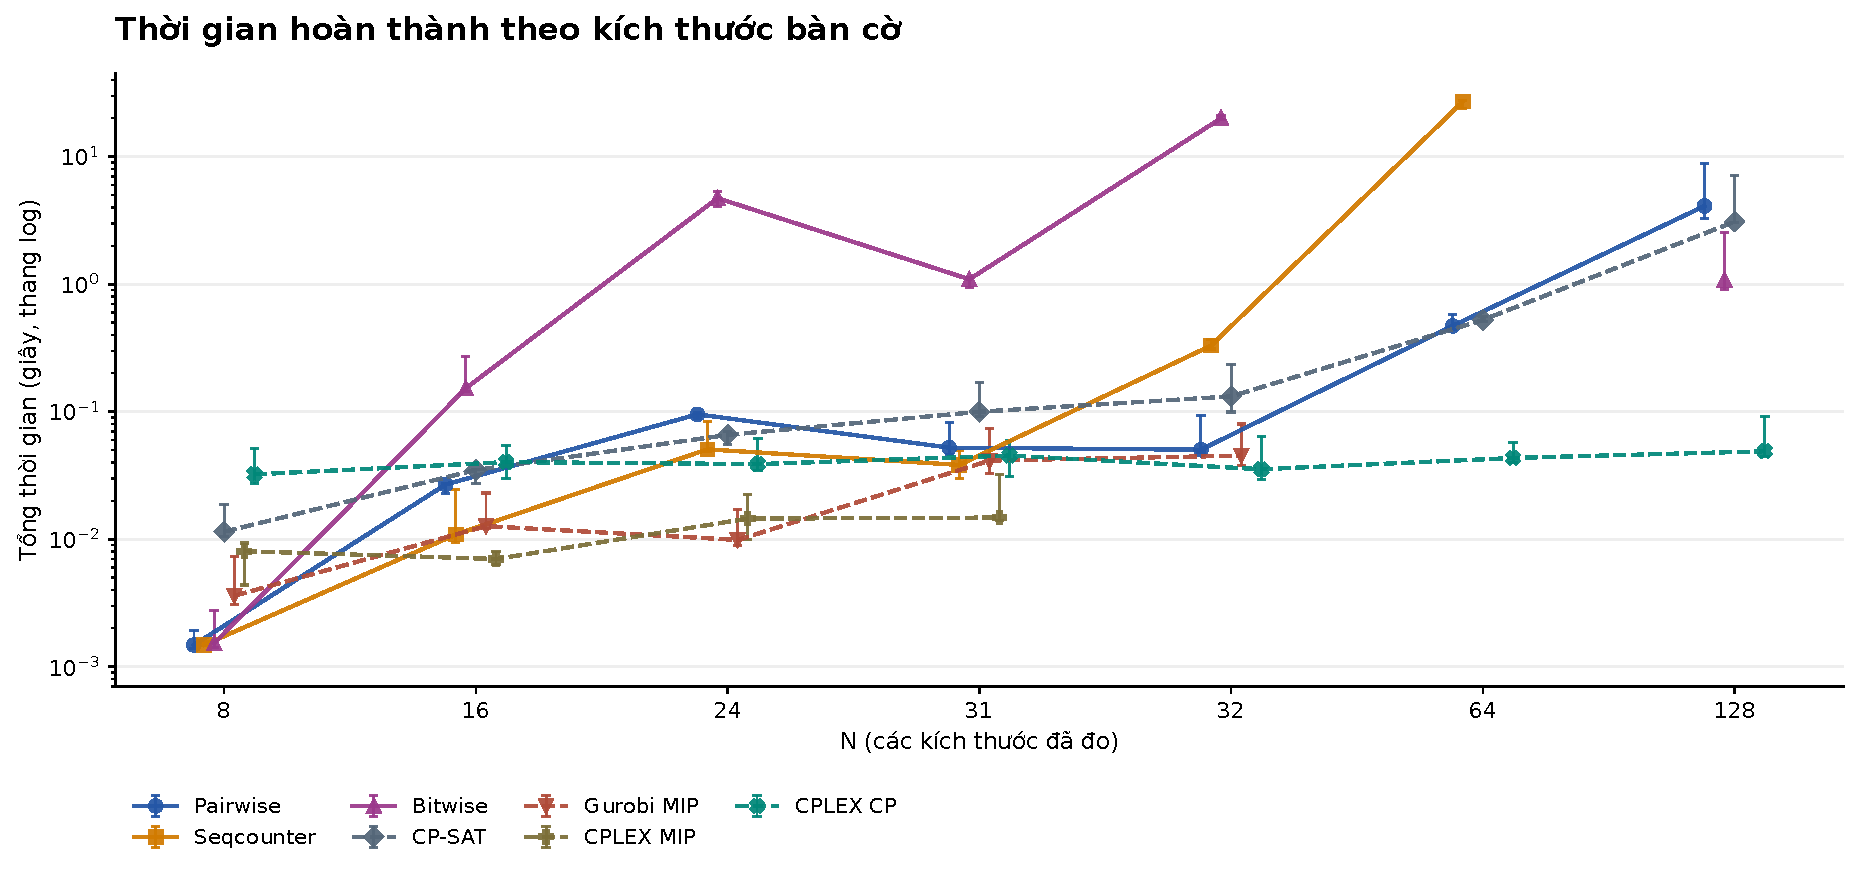
\includegraphics[width=\linewidth]{figures/01_total_time.pdf}
\caption{Trung vị tổng thời gian; thanh sai số là nhỏ nhất--lớn nhất của năm lượt. Trục tung logarithm. Các giá trị $N$ là nhãn phân loại có khoảng cách đều, không phải trục số tuyến tính; các đường được dịch ngang nhẹ để dễ đọc. Ô \TO/\GL{} không có điểm thời gian và làm ngắt đường nối.}\label{fig:total}
\end{figure}

Pairwise hoàn thành tất cả 35 lượt SAT. Sequential counter hoàn thành ở $N=64$ nhưng trung vị tổng thời gian 27,011 giây, khoảng 57,34 lần pairwise tại cùng $N$; tới $N=128$ nó hết hạn cả năm lượt. Bitwise hết hạn cả năm lượt ở $N=64$ nhưng lại hoàn thành $N=128$ với trung vị khoảng 1,074 giây. Dữ liệu chứng minh sự không đơn điệu trong cấu hình khảo sát; nó không xác định nguyên nhân riêng lẻ của hiện tượng đó.

Trong nhóm đối chứng, Gurobi MIP có trung vị thấp nhất tại $N=24$ và CPLEX MIP tại $N=16,31$. CP Optimizer có trung vị thấp nhất trong các cấu hình đã chạy ở $N=32,64,128$. Tại hai kích thước sau, cả hai MIP đều thiếu dữ liệu vì giấy phép; không thể từ bảng này kết luận CP Optimizer nhanh hơn các bản MIP không bị giới hạn tại những kích thước ấy.

\subsection{Kích thước CNF và quan hệ với thời gian}
\begin{table}[htbp]
\caption{Số biến xuất hiện trong CNF (V) và số mệnh đề được dựng (C).}\label{tab:cnf}
\centering\footnotesize\setlength{\tabcolsep}{5pt}
\begin{tabular}{rrrrrrr}
\toprule
$N$ & Pairwise V & Pairwise C & Seqcounter V & Seqcounter C & Bitwise V & Bitwise C \\
\midrule
8 & 64 & 744 & 270 & 600 & 170 & 724 \\
16 & 256 & 6\,352 & 1\,182 & 2\,728 & 568 & 3\,924 \\
24 & 576 & 21\,944 & 2\,734 & 6\,392 & 1\,158 & 10\,820 \\
31 & 961 & 47\,802 & 4\,617 & 10\,858 & 1\,753 & 18\,534 \\
32 & 1\,024 & 52\,640 & 4\,926 & 11\,592 & 1\,846 & 19\,796 \\
64 & 4\,096 & 428\,864 & 20\,094 & 47\,752 & 6\,132 & 95\,572 \\
128 & 16\,384 & 3\,462\,784 & 81\,150 & 193\,800 & 21\,234 & 447\,828 \\
\bottomrule
\end{tabular}
\tabnote{V bao gồm biến gốc và biến phụ. Các số đếm của cùng một cấu hình không đổi qua năm lượt.}
\end{table}

\begin{figure}[htbp]
\centering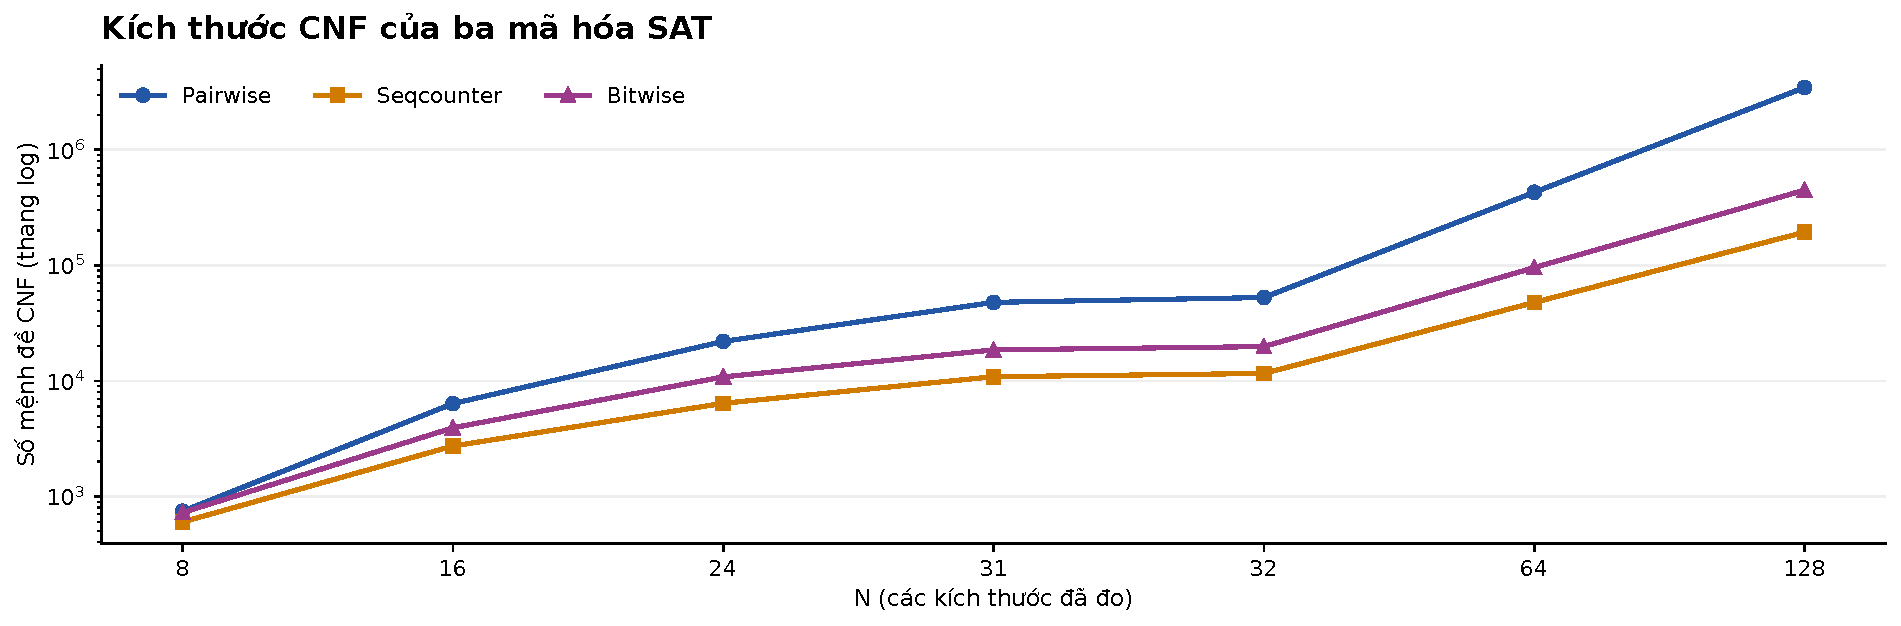
\includegraphics[width=.92\linewidth]{figures/02_cnf_size.pdf}
\caption{Số mệnh đề CNF được sinh trước khi nạp vào solver. Trục tung logarithm; các nhãn $N$ cách đều. Số đếm tại ô timeout vẫn tồn tại vì pha dựng và thống kê mô hình đã hoàn thành trước pha giải.}\label{fig:cnf}
\end{figure}

Bảng~\ref{tab:cnf} phản ánh đúng xu hướng quy mô ở Mục~\ref{sec:sat}: pairwise không thêm biến phụ nhưng số mệnh đề tăng nhanh; sequential counter tạo nhiều biến phụ hơn nhưng CNF ngắn hơn. Tại $N=128$, pairwise có 3\,462\,784 mệnh đề, bitwise 447\,828 và sequential counter 193\,800. Pairwise nhiều mệnh đề hơn sequential counter khoảng 17,87 lần, trong khi sequential counter lại hết thời gian.

Điều này bác bỏ quy tắc đơn giản ``ít mệnh đề hơn thì luôn giải nhanh hơn'' trên chính bộ dữ liệu này. Kích thước CNF chi phối việc dựng và nạp, nhưng đường tìm kiếm còn phụ thuộc vào cấu trúc các mệnh đề, biến phụ và quyết định của solver. Đây là cách diễn giải phù hợp với quan sát, chưa phải phân tích nhân quả: thí nghiệm chưa ghi đủ số xung đột, quyết định, lan truyền hay khởi động lại để xác định cơ chế gây ra từng chênh lệch.

\subsection{Phân rã thời gian tại $N=128$}
\begin{table}[htbp]
\caption{Trung vị từng pha tại $N=128$, đơn vị ms; chỉ các cấu hình có 5/5 SAT.}\label{tab:phases}
\centering\small
\begin{tabular}{lrrrrr}
\toprule
Phương pháp & Dựng & Khởi tạo & Giải & Hậu xử lý & Tổng \\
\midrule
SAT pairwise & 2\,294.487 & 1\,725.828 & 57.602 & 1.085 & 4\,106.107 \\
SAT bitwise & 198.960 & 248.993 & 618.740 & 1.449 & 1\,073.782 \\
CP-SAT & 3.827 & 0.055 & 3\,089.983 & 0.487 & 3\,094.220 \\
CP Optimizer & 1.835 & 26.513 & 18.620 & 0.180 & 49.009 \\
\bottomrule
\end{tabular}
\tabnote{Trung vị từng cột được tính độc lập; tổng các trung vị thành phần không nhất thiết bằng trung vị tổng.}
\end{table}

\begin{figure}[htbp]
\centering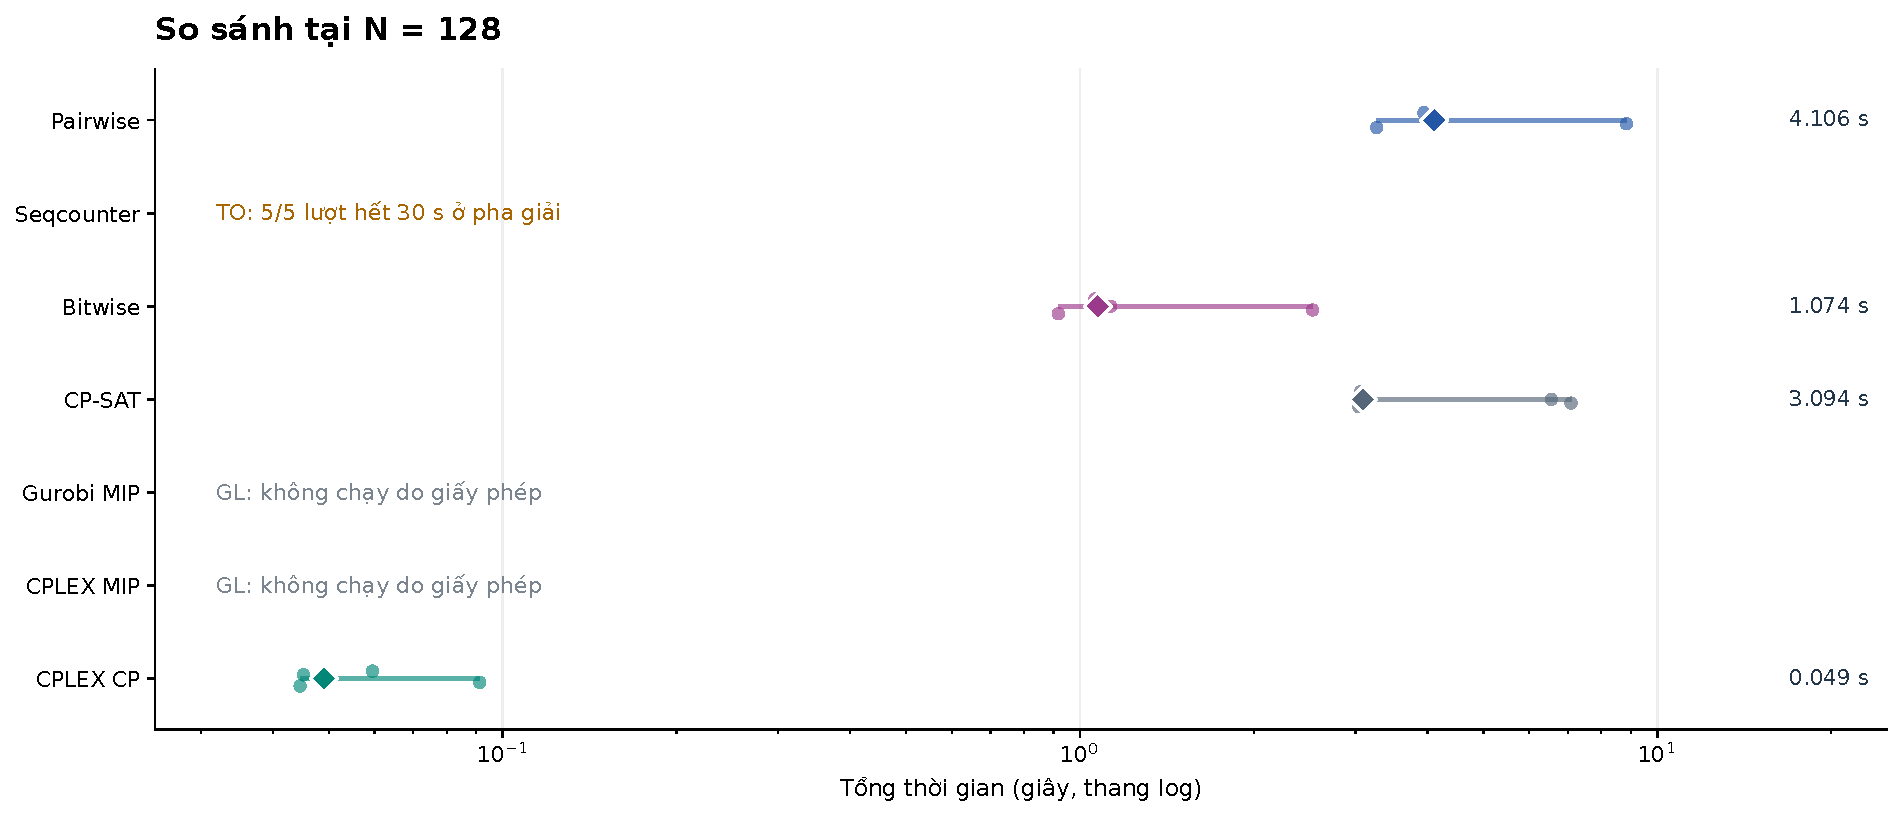
\includegraphics[width=.92\linewidth]{figures/03_n128_detail.pdf}
\caption{Chi tiết tổng thời gian tại $N=128$. Các chấm là từng lượt; hình thoi là trung vị và đoạn ngang là khoảng nhỏ nhất--lớn nhất. Trục thời gian logarithm; nhãn timeout và giấy phép không được vẽ như giá trị thời gian giả.}\label{fig:n128}
\end{figure}

Pairwise có trung vị pha giải khoảng 57,602 ms, nhưng trung vị tổng thời gian là 4\,106,107 ms. Trung vị của tỷ lệ $(t_{\mathrm{build}}+t_{\mathrm{init}})/t_{\mathrm{total}}$, tính riêng trên từng lượt, bằng 98,51\%. Như vậy nút thắt quan sát được của pairwise ở $N=128$ là dựng và nạp CNF. Chỉ công bố thời gian lời gọi giải sẽ bỏ qua phần lớn chi phí sử dụng cấu hình này.

Bitwise cần nhiều thời gian hơn trong API giải so với pairwise tại $N=128$, nhưng có CNF nhỏ hơn và tổng thời gian thấp hơn khoảng 3,82 lần. CP-SAT có chi phí dựng/khởi tạo phía Python nhỏ, còn phần lớn tổng thời gian của nó nằm trong API giải. CP Optimizer đạt trung vị tổng 49,009 ms; khoảng nhỏ nhất--lớn nhất là 44,583--91,284 ms. Với cùng $N$, khoảng của pairwise là 3,265--8,842 giây và bitwise là 0,917--2,529 giây. Toàn bộ các lượt được giữ lại, không suy đoán lượt chậm là do một nguyên nhân hệ thống cụ thể khi chưa có số đo hỗ trợ.

\subsection{Giới hạn của kết luận}\label{sec:limitations}
Kết quả cần được đọc trong các giới hạn sau. Thứ nhất, tập thí nghiệm chỉ có bảy bàn cờ chuẩn, đều biết là có nghiệm; chưa có Completion, ô cấm, đếm nghiệm hoặc bộ dữ liệu UNSAT lớn. Vì thế tỷ lệ SAT cao không chứng minh hiệu quả trên bài toán ràng buộc tổng quát.

Thứ hai, chỉ một máy và một cấu hình seed được khảo sát. Năm lần lặp giúp mô tả biến thiên khi chạy lại, không tạo căn cứ cho kiểm định trên một quần thể bài toán. Kích thước $N$ được chạy tăng dần nên vẫn có khả năng tương quan với trạng thái máy theo thời gian; nhiệt độ, xung nhịp và tải nền không được ghi. Báo cáo không công bố khoảng tin cậy hay khẳng định thứ hạng thống kê có ý nghĩa.

Thứ ba, việc so sánh đồng thời thay cả solver và cách biểu diễn. CP dùng $N$ biến miền hữu hạn cùng AllDifferent, còn SAT/MIP dùng $N^2$ biến ô. Do đó kết quả đánh giá \emph{tổ hợp mô hình--backend--giao diện}; không đủ để quy mọi ưu thế cho một thuật toán bên trong solver. Giới hạn giấy phép còn làm thiếu các phép đo MIP lớn.

Cuối cùng, chưa đo bộ nhớ đỉnh. Số mệnh đề lớn của pairwise gợi ý cần khảo sát chi phí bộ nhớ, nhưng không thể suy từ số đếm CNF ra lượng RAM thực dùng. Giới hạn giải 30 giây chỉ cho biết một cấu hình chưa trả kết quả trong hạn, không cho biết thời gian cuối cùng nó cần để hoàn thành.
\FloatBarrier

\section{Kết luận và hướng phát triển}\label{sec:conclusion}
Bài tập đã xây dựng mô hình SAT cho N-Queens với ba mã hóa AMO, cơ chế giải mã và kiểm tra nghiệm, đồng thời thực nghiệm với CP-SAT, CP Optimizer, CPLEX MIP và Gurobi MIP. Đợt đo chính có 210 nghiệm hợp lệ trên 220 lời gọi solver; 10 lượt hết hạn được giữ đúng là UNKNOWN và 25 lượt không chạy được tách riêng theo chính sách giấy phép.

Trong phạm vi khảo sát, không có mã hóa SAT thống trị ở mọi kích thước. Pairwise hoàn thành toàn bộ các lượt, sequential counter tạo CNF nhỏ nhưng hết hạn ở $N=128$, còn bitwise có tổng thời gian tốt nhất trong nhóm SAT tại $N=128$. Phân rã thời gian cho thấy việc dựng và nạp CNF có thể quyết định kết quả so sánh; số mệnh đề ít hơn không bảo đảm thời gian giải ngắn hơn.

Hướng phát triển gồm bổ sung các biến thể có quân hậu đặt trước hoặc ô cấm, khảo sát nhiều seed, đo bộ nhớ và thống kê CDCL, đánh giá phá vỡ đối xứng, và mở rộng so sánh MIP khi có giấy phép phù hợp. Các thay đổi này cần được thực nghiệm như những cấu hình mới, giữ riêng với bộ số liệu hiện tại.

\section*{Data Availability}
Dữ liệu gốc của đợt chạy gồm \code{measurements.csv}, \code{warmup.csv} và \code{manifest.json}. Mã đợt chạy là \code{main_v1_20261016_224847_037042}. Gói mã nguồn báo cáo kèm nguyên tệp ZIP dữ liệu, bảng tổng hợp, kết quả kiểm tra và script \code{analyze_results.py}. Thông tin môi trường, lịch chạy, chính sách giấy phép và SHA-256 của tám tệp nguồn được lưu trong manifest.

\noindent\textbf{Mã nguồn dự án:} \ShowCodeURL\par
\noindent\textbf{Dữ liệu thực nghiệm thô:} \ShowDataURL\par
Hai liên kết trên chưa được cung cấp ở thời điểm soạn bản thảo; cần cập nhật bằng địa chỉ truy cập thật trong \code{config.tex} trước khi nộp. Mã băm nhận diện bản mã đã chạy, nhưng không thay thế việc cung cấp các tệp nguồn tương ứng. Gói LaTeX của báo cáo không được xem là toàn bộ mã nguồn solver.

\appendix
\section{Tái lập và đối chiếu kết quả}\label{app:reproduce}
\subsection{Chạy lại phép đo}
Trong thư mục dự án có đủ các mô-đun ở Bảng~\ref{tab:modules}, cấu hình lệnh PowerShell tương ứng với đợt đo là:
\begin{Verbatim}[fontsize=\small,breaklines=true,frame=single]
.\.venv\Scripts\python.exe benchmark_main.py --plan
.\.venv\Scripts\python.exe benchmark_main.py `
  --group all --repeats 5 --solve-limit 30 --setup-limit 120 `
  --cpu-name "Intel Core i7-10610U" --ram-gb 15.8
\end{Verbatim}
Khi tái lập trên máy khác, cần thay tên CPU và RAM bằng thông tin máy thực tế. Các phiên bản Python và thư viện được liệt kê ở Bảng~\ref{tab:environment}. Lệnh không tự cấp giấy phép MIP; chính sách giới hạn kích thước vẫn áp dụng. Một lần chạy mới tạo dữ liệu mới và không được kỳ vọng cho thời gian giống tuyệt đối.

\subsection{Tổng hợp lại dữ liệu đã có}
Trong thư mục gốc của gói LaTeX, chạy lệnh dưới đây bằng Python; script phân tích chỉ dùng thư viện chuẩn và không gọi lại solver:
\begin{Verbatim}[fontsize=\small,breaklines=true,frame=single]
python tools/analyze_results.py data/main_v1_20261016_224847_037042.zip --output analysis_recheck
\end{Verbatim}
Script kiểm tra lịch, trạng thái, nghiệm và tính nhất quán các pha, rồi xuất \code{analysis.json} và \code{summary.csv}. Đơn vị thời gian trong hai tệp này là giây; các bảng của bài báo đổi sang mili giây. Trung vị tính trên năm lượt của mỗi ô; dữ liệu warm-up không tham gia.

\subsection{Nhận diện dữ liệu}
SHA-256 của tệp ZIP gốc là:
\begin{Verbatim}[fontsize=\small,breaklines=true]
a005c1453c1a3811f8d77623cb3a954c53912669b945b7bcb9420f6193e7dffe
\end{Verbatim}
Đây là dấu nhận diện để phát hiện khác biệt byte của tệp, không phải chứng nhận độc lập rằng mọi nội dung trong tệp đúng. Bảng~\ref{tab:wall} bổ sung trung vị thời gian toàn tiến trình tại $N=128$ để người đọc phân biệt với chỉ số chính $t_{\mathrm{total}}$.
\begin{table}[htbp]
\caption{Hai phạm vi đo khác nhau tại $N=128$, trung vị năm lượt (ms).}\label{tab:wall}
\centering\small
\begin{tabular}{lrr}
\toprule
Phương pháp & $t_{\mathrm{total}}$ & \code{process_wall_s} \\
\midrule
SAT pairwise & 4\,106.107 & 5\,072.776 \\
SAT bitwise & 1\,073.782 & 1\,375.466 \\
CP-SAT & 3\,094.220 & 4\,078.751 \\
CP Optimizer & 49.009 & 912.675 \\
\bottomrule
\end{tabular}
\tabnote{Cột cuối bao gồm khởi động tiến trình, import, thống kê, giao tiếp và thu hồi; đã đổi từ giây sang ms.}
\end{table}


\bibliographystyle{cas-model2-names}
\begingroup\raggedright
\bibliography{references}
\endgroup
\end{document}
